\documentclass{beamer}
\usetheme{metropolis}
\usepackage{graphicx}
\usepackage{subfig}
\usepackage{tcolorbox}
\title{Calculus-Based Physics-2: Electricity, Magnetism, and Thermodynamics (PHYS180-02): Unit 1}
\author{Jordan Hanson}
\institute{Whittier College Department of Physics and Astronomy}

\begin{document}
\maketitle

\section{Unit 0 Review}

\begin{frame}{Unit 0 Review}
\textit{Physics} - $\phi\upsilon\sigma\iota\kappa\acute{\eta}$ - "phusik\'e": \textit{knowledge of nature} \\
from $\phi\acute{\upsilon}\sigma\iota\varsigma$ - "ph\'usis": \textit{nature} \\
\textbf{Reading: Chapters 1 and 2 (for Unit 1)}
\begin{enumerate}
\item Estimation/Approximation
\begin{itemize}
\item \alert{Estimating} the correct order of magnitude
\item \alert{Building} complex quantities
\item \alert{Unit analysis}
\end{itemize}
\item Review of concepts from Newtonian mechanics
\begin{itemize}
\item Kinematics and \alert{Newton's Laws}
\item Work-energy theorem, energy conservation
\item Momentum, conservation of momentum
\end{itemize}
\end{enumerate}
\end{frame}

\begin{frame}{Unit 0 Review}
Two molucules collide elastically.  Which of the following is true?
\begin{itemize}
\item A: Both potential energy and momentum are conserved for each molecule
\item B: Only the momentum is conserved for each molecule
\item C: Momentum and kinetic energy are conserved for each molecule
\item D: Neither momentum nor energy is conserved for each molecule
\end{itemize}
\end{frame}

\begin{frame}{Unit 0 Review}
Suppose a molecule is headed towards the wall of a container with speed $v$ and mass $m$.  If it collides elastically with the wall and returns in the exact same direction from which it came, what is the change in momentum of the molecule?
\begin{itemize}
\item A: $mv$
\item B: $\frac{1}{2}mv^2$
\item C: $mv^2$
\item D: $2mv$
\end{itemize}
\end{frame}

\begin{frame}{Unit 0 Review}
Do you remember how to take the derivative of an exponential function?  Let $f(t) = \exp(\alpha t)$.  What is $f'(t)$?
\begin{itemize}
\item A: $\exp(\alpha t)$
\item B: $\alpha\exp(\alpha t)$
\item C: $\exp(\alpha t)/\alpha$
\item D: $\exp(2\alpha t)$
\end{itemize}
\end{frame}

\begin{frame}{Unit 0 Review}
What about multiplying exponentials?  What is $f(t)g(t)$, if $f(t) = \exp(\alpha t)$ and $g(t) = \exp(\beta t)$?
\begin{itemize}
\item A: $\exp(\alpha\beta t)$
\item B: $\exp(\frac{\alpha}{\beta} t)$
\item C: $\exp(\frac{\beta}{\alpha} t)$
\item D: $\exp((\alpha+\beta) t)$
\end{itemize}
\end{frame}

\section{Unit 1 Summary}

\begin{frame}{Unit 1 Summary}
\textbf{Reading: Chapters 1 and 2}
\begin{enumerate}
\item Temperature, Heat, and the 0th Law of Thermodynamics
\item Heat flow and transfer mechanisms
\item Kinetic Theory of Gases
\end{enumerate}
\end{frame}

\section{JITT - Reading Quiz Results}

\begin{frame}{JITT - Reading Quiz Results}
\begin{enumerate}
\item In your own words, what is the cause of thermal expansion, and how is thermal expansion in three dimensions tied to thermal expansion in one dimension (linear expansion)?
\item Describe in your own words the difference between two objects with different emissivities, as emissivity is related to the Stefan-Boltzmann equation.
\item Describe in your own words the role of Boltzmann's constant and Avogadro's number in thermodynamics.
\end{enumerate}
\end{frame}

\begin{frame}{JITT 1.1 Question 1}
\small
The cause of thermal expansion is a change in temperature, thermal expansion in three dimensions is tied to thermal expansion in one dimension because they are similar equations when solving them, one just deals with a single length and the other deals with a volume and a multiple of 3 (Its late and I can’t think of a way to connect them outside of one of them is in one dimension and the other is in 3 dimensions, so I looked at the formulas for solving them).
\begin{enumerate}
\item What is correct about this statement?
\item How can we improve the correctness?
\end{enumerate}
\end{frame}

\begin{frame}{JITT 1.1 Question 1}
\small
Thermal expansion is caused when molecules are heated and start to get "energize" and spread out and bonds break or loosen. Objects expand in all directions, and linear expansion changes in length, which could be tied to a particular direction. 
\begin{enumerate}
\item What is correct about this statement?
\item How can we improve the correctness?
\end{enumerate}
\end{frame}

\begin{frame}{JITT 1.1 Question 1}
\textbf{Things to consider:} 
\begin{enumerate}
\item The asymmetry of the molecular (Leonard-Jones) potential.
\item One and three dimensional versions of Equation 1.1 in the text.
\end{enumerate}
\end{frame}

\begin{frame}{JITT 1.1 Question 2}
\small
Under the same temperature and wavelength conditions an object that emitts more energy relative to a blackbody has a greater emissivity as the temperatures of the objects increase, their emissivities do as well.
\begin{enumerate}
\item What is correct about this statement?
\item How can we improve the correctness?
\end{enumerate}
\end{frame}

\begin{frame}{JITT 1.1 Question 2}
\small
The two objects with different emissivities will have two different absolute temperatures, as the absolute temperature is proportionate to emissivity.
\begin{enumerate}
\item What is correct about this statement?
\item How can we improve the correctness?
\end{enumerate}
\end{frame}

\begin{frame}{JITT 1.1 Question 2}
\small
Emissivity is the property of an object to absorb and emit thermal radiation. Black being a better emitter and absorber than colors such as white or gray. Radiation is also emitted from all parts of an object, so a greater surface area means more emission. this can be calculated with the Stefan-Boltzmann equation.
\begin{enumerate}
\item What is correct about this statement?
\item How can we improve the correctness?
\end{enumerate}
\end{frame}

\begin{frame}{JITT 1.1 Question 2}
\textbf{Things to consider:} 
\begin{enumerate}
\item $\sigma e A T^4$ versus $\sigma e A \left( T_2^4 - T_1^4 \right)$.
\item Heat and color as an indication of temperature (we can do this with stars, for example).
\end{enumerate}
\end{frame}

\begin{frame}{JITT 1.1 Question 3}
\small
Avagardos number ($6.02 \times 10^{23}$) relates the mass of an object to the number of its neutrons and protons since they should roughly be the same as the total mass. Boltzmann's constant ($1.38 \times 10^{-23}$) is used in the ideal gas law which describes how a gas acts when the desnity is too low or the temperature is so high that the gas is far from becoming a liquid.
\begin{enumerate}
\item What is correct about this statement?
\item How can we improve the correctness?
\end{enumerate}
\end{frame}

\begin{frame}{JITT 1.1 Question 3}
\small
Both Boltzmann’s constant and Avogadro’s number are used In many equations involving thermodynamics.  (it was a difficult reading to understand and I’d appreciate it if we could briefly go over some of it in class and identify the most important parts of it to help me better understand, thanks!) 
\begin{enumerate}
\item This is \textit{good.}  Admitting we don't know is good.
\item How would you describe the role of Boltzmann's constant in the ideal gas law?
\item How would you describe the role of Avogadro's number in the ideal gas law?
\end{enumerate}
\end{frame}

\section{Temperature, Heat, and the 0th Law of Thermodynamics}

\begin{frame}{Temperature, Heat, and the 0th Law of Thermodynamics}
\begin{figure}
\centering
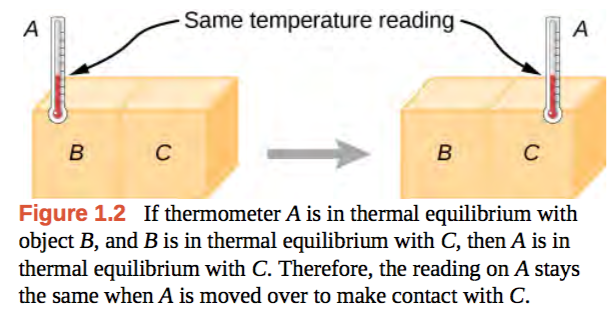
\includegraphics[width=0.9\textwidth,trim=0cm 4cm 0cm 0cm,clip=true]{figures/zero.png}
\caption{\label{fig:zero} The zeroeth law of thermodynamics.  We need this idea to have a firm understanding of temperature readings, because a \textbf{thermometer} is itself a thermal system.}
\end{figure}
\end{frame}

\begin{frame}{Temperature, Heat, and the 0th Law of Thermodynamics}
\begin{figure}
\centering
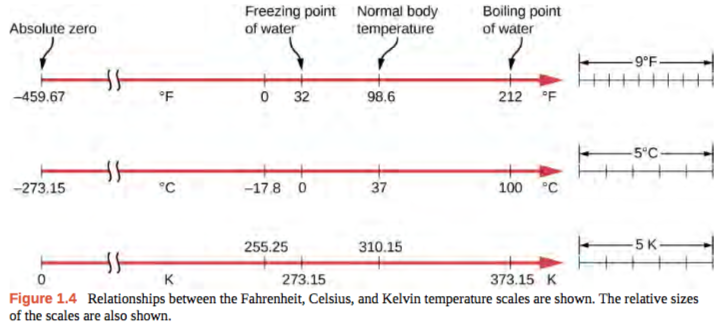
\includegraphics[width=0.95\textwidth,trim=0cm 1.5cm 0cm 0cm,clip=true]{figures/temp1.png}
\caption{\label{fig:temp1} Three temperature scales.}
\end{figure}
\end{frame}

\begin{frame}{Temperature, Heat, and the 0th Law of Thermodynamics}
\begin{figure}
\centering
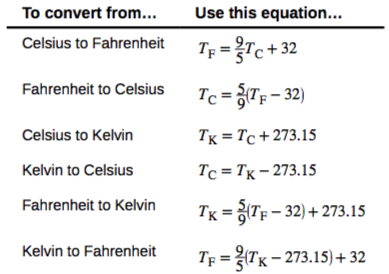
\includegraphics[width=0.6\textwidth]{figures/temp2.png}
\caption{\label{fig:temp2} Three temperature scales.  The Fahrenheit scale places 0 for a solution of brine and ice, with 180 degrees between freezing and boiling of water.  Celsius scale has 0 for freezing and 100 for boiling.  Absolute zero of Kelvin scale will be discussed below.}
\end{figure}
\end{frame}

\begin{frame}{Temperature, Heat, and the 0th Law of Thermodynamics}
Suppose the temperature of a system is raised by 10$^{\circ}$ F.  Which of the following is true?
\begin{itemize}
\item A: The increase is more than 10 degrees in $^{\circ}$C.
\item B: The increase is smaller than 10 degrees in $^{\circ}$C.
\item C: The increase is the same in $^{\circ}$C.
\item D: Depends on the initial temperature in $^{\circ}$F.
\end{itemize}
\end{frame}

\begin{frame}{Temperature, Heat, and the 0th Law of Thermodynamics}
Suppose the temperature of a system is raised by 10$^{\circ}$C.  Which of the following is true?
\begin{itemize}
\item A: The increase is more than 10 degrees in $^{\circ}$K.
\item B: The increase is smaller than 10 degrees in $^{\circ}$K.
\item C: The increase is the same in $^{\circ}$K.
\item D: Depends on the initial temperature in $^{\circ}$C.
\end{itemize}
\end{frame}

\begin{frame}{Temperature, Heat, and the 0th Law of Thermodynamics}
The formula for conversion from Celcius temperature to Fahrenheit temperatures is $T_{\rm F} = \frac{9}{5}T_{\rm C} + 32$.  Which of the following is true?
\begin{itemize}
\item A: $0^{\circ}-10^{\circ}$C is comparable to room temperature
\item B: $35^{\circ}-40^{\circ}$C is comparable to human body temperature
\item C: $30^{\circ}-35^{\circ}$C is comparable to human body temperature
\item D: $15^{\circ}-20^{\circ}$C outdoors would correspond to hot weather
\end{itemize}
\end{frame}

\begin{frame}{Temperature, Heat, and the 0th Law of Thermodynamics}
How do thermometers work?  What is temperature, really?  \textit{Temperature is a macroscopic indication of microscopic kinetic energy}.  We need the idea of \textbf{thermal expansion}: \\ 
\begin{equation}
\frac{dL}{dT} = \alpha L
\label{eq:linear}
\end{equation}
In Eq. \ref{eq:linear}, $T$ is the temperature, $L$ is the length of an object, and $\alpha$ is the coefficient of linear thermal expansion, in units of inverse degrees.
\end{frame}

\begin{frame}{Temperature, Heat, and the 0th Law of Thermodynamics}
\begin{figure}
\centering
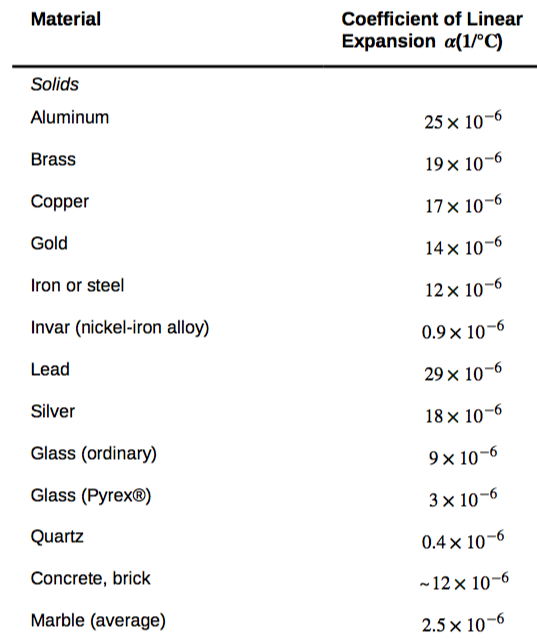
\includegraphics[width=0.5\textwidth]{figures/linear.png}
\caption{\label{fig:linear} Linear thermal expansion coefficients.}
\end{figure}
\end{frame}

\begin{frame}{Temperature, Heat, and the 0th Law of Thermodynamics} 
\begin{equation}
\frac{dL}{dT} = \alpha L
\label{eq:linear2}
\end{equation}
Equation \ref{eq:linear2} is a differential equation with a particular solution:
\begin{equation}
L(T) = L_{\rm 0}\exp(\alpha T) \label{eq:exp}
\end{equation}
We've seen that in practice, $\alpha$ values are small.  In this case we may approximate:
\begin{align}
L(T)/L_{\rm 0} &\approx 1+\alpha T \\
\Delta L &\approx \alpha L_{\rm 0} \Delta T \label{eq:linear3}
\end{align}
Equation \ref{eq:linear3} is the equation found in Chapter 1 of the reading.
\end{frame}

\begin{frame}{Temperature, Heat, and the 0th Law of Thermodynamics}
\begin{figure}
\centering
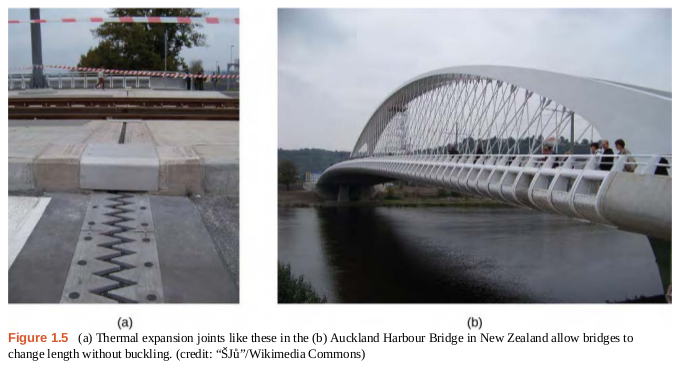
\includegraphics[width=0.9\textwidth]{figures/bridge.png}
\caption{\label{fig:bridge} Bridge expansion joints.}
\end{figure}
\end{frame}

\begin{frame}{Temperature, Heat, and the 0th Law of Thermodynamics} 
Chapter 1 also contains these formulae for two and three-dimensional expansion:
\begin{align}
\Delta A &\approx 2\alpha A_{\rm 0} \Delta T \label{eq:linear4} \\
\Delta V &\approx 3\alpha V_{\rm 0} \Delta T \label{eq:linear5}
\end{align}
Why?  Properties of exponentials.  \textbf{Group board exercise}: prove Eq. \ref{eq:linear5} using Eq. \ref{eq:exp}.
\end{frame}

\begin{frame}{Temperature, Heat, and the 0th Law of Thermodynamics}
\small
\textit{Pipe Transport}: Some oil and gasoline pipelines are above ground, exposed to the elements.  The coefficient of thermal volumetric expansion for gasoline is much larger than that of steel.  Why would it be a bad idea to completely fill a pipeline with gasoline, knowing there will be large temperature variations?
\begin{itemize}
\item A: For large increases in temperature, the pipeline expands more rapidly than gasoline, leaving gaps for leaks.
\item B: For large increases in temperature, the gasoline expands more rapidly than the pipeline, building pressure and causing pipeline bursts.
\item C: For large decreases in temperature, the gasoline shrinks more rapidly than the pipeline, building pressure and causing pipeline bursts.
\item D: None of these.
\end{itemize}
\end{frame}

\begin{frame}{Temperature, Heat, and the 0th Law of Thermodynamics}
If an object has a length of 10 cm, and a linear thermal expansion coefficient of $100 \times 10^{-6}$ 1/$^{\circ}$C, what is the change in length of the object if the temperature is increased from 0 $^{\circ}$C to 100 $^{\circ}$C?
\begin{itemize}
\item A: 0.1 mm
\item B: 1 mm
\item C: 1 cm
\item D: 10 cm
\end{itemize}
\end{frame}

\begin{frame}{Temperature, Heat, and the 0th Law of Thermodynamics}
Recall from last semester that we studied \textit{stress} and \textit{strain}:
\begin{align}
\frac{F}{A} &= Y \frac{\Delta L}{L} \\
stress &= Y \times strain
\end{align}
Now we can predict strain from temperature changes, and make statements about the implied \textit{thermal stresses}.  This is important for mechanical engineering designs.
\begin{equation}
\frac{F}{A} = Y \alpha \Delta T
\end{equation}
\end{frame}

\begin{frame}{Temperature, Heat, and the 0th Law of Thermodynamics}
\begin{equation}
\frac{F}{A} = Y \alpha \Delta T
\end{equation}
\textit{Steel pipeline design}: Suppose a steel pipeline ($\alpha = 12 \times 10^{-6}$ 1/$^{\circ}$C, $Y = 30\times 10^{9}$ N/m$^2$) is designed and built at temperatures of 30 $^{\circ}$C, but experiences temperatures of 0 $^{\circ}$C.  What stress does the pipeline experience at the attachment point?
\begin{itemize}
\item A: -0.1 MPa
\item B: 1 MPa
\item C: -10 MPa
\item D: 100 MPa
\end{itemize}
\textit{Is the pipeline pulling or pushing on the attachment point?}
\end{frame}

\begin{frame}{Temperature, Heat, and the 0th Law of Thermodynamics}
\begin{figure}
\centering
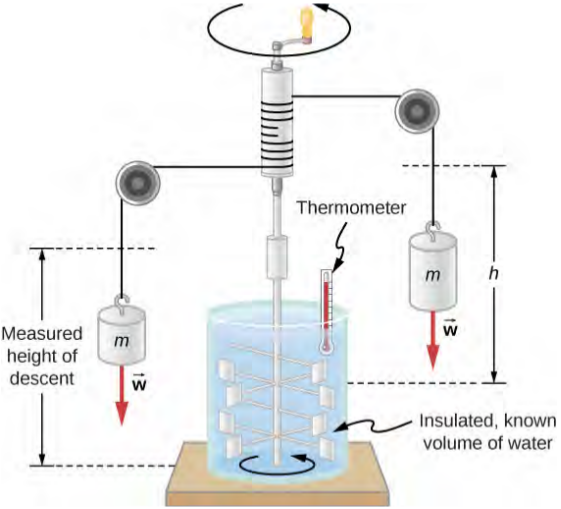
\includegraphics[width=0.5\textwidth]{figures/Joule.png}
\caption{\label{fig:Joule} Demonstrating that work and heat are equivalent (paper topic from last semester).}
\end{figure}
\end{frame}

\begin{frame}{Temperature, Heat, and the 0th Law of Thermodynamics}
Which of the following is true, regarding Fig. \ref{fig:Joule}?
\begin{itemize}
\item A: The temperature increase is proportional to the decrease in height of the masses.
\item B: The temperature increase is proportional to $g$.
\item C: A and B
\item D: None of these
\end{itemize}
\end{frame}

\begin{frame}{Temperature, Heat, and the 0th Law of Thermodynamics}
Regarding Fig. \ref{fig:Joule}, if total mass is 1.0 kg (two 0.5 kg masses), $g = 10$ m/s$^2$, and $h = 1$ m, what is the temperature increase in the water?
\begin{itemize}
\item A: 10 J
\item B: 10 $^{\circ}$K
\item C: 10 $^{\circ}$C
\item D: Cannot determine
\end{itemize}
\end{frame}

\begin{frame}{Temperature, Heat, and the 0th Law of Thermodynamics}
The heat required to obtain a change in temperature is proportional to the mass of the substance to be heated (obvious if you understand heat to be caused by motions of molecules).  The coefficient is called the \textit{specific heat capacity}:
\begin{equation}
Q = mc\Delta T
\end{equation}
More generally,
\begin{equation}
c = \frac{1}{m}\frac{dQ}{dT}
\end{equation}
Units: Joules per unit temperature per unit mass (J/(kg C)).  1 \textit{calorie} is the energy required to heat 1 gram of water 1 degree C.  For food, 1 kcal = 1 Calorie $\rightarrow$ endless debates about food science...
\end{frame}

\begin{frame}{Temperature, Heat, and the 0th Law of Thermodynamics}
\begin{figure}
\centering
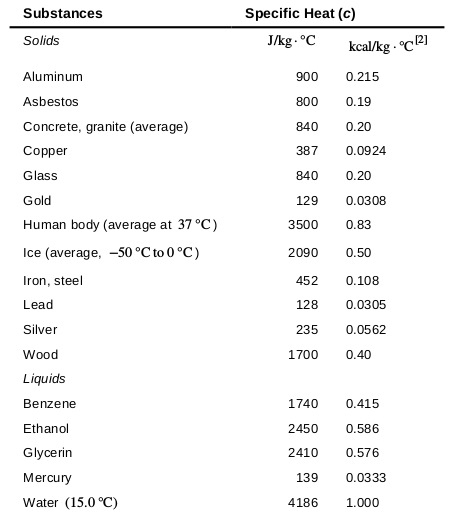
\includegraphics[width=0.5\textwidth]{figures/c.png}
\caption{\label{fig:c} Notice how water is on a different scale than most other substances.}
\end{figure}
\end{frame}

\begin{frame}{Temperature, Heat, and the 0th Law of Thermodynamics}
A 0.500 kg aluminum pan on a stove and 0.250 L of water in it are heated from 20.0 $^\circ$C to 80.0 $^\circ$C. a) How much heat is required? What percentage of the heat is used to raise the temperature of b) the pan and c) the water? \\ \vspace{0.5cm}
\textbf{Group board exercise}: $c_{\rm W} = 4186$ J/kg/C and $c_{\rm Al} = 900$ J/kg/C.
\end{frame}

\begin{frame}{Temperature, Heat, and the 0th Law of Thermodynamics}
For a thermodynamically isolated system, we have
\begin{equation}
Q_{\rm cold} + Q_{\rm hot} = 0
\label{eq:calor}
\end{equation}
That is, if heat is conserved, the heat lost by a hot system is equal and opposite to the heat gained by the cold object. This sort of balancing is known as \textit{calorimetry}.  \\ \vspace{0.5cm}
Es como la palabra ``calor'' en espa\~{n}ol: hace calor hoy.
\end{frame}

\begin{frame}{Temperature, Heat, and the 0th Law of Thermodynamics}
\small
Suppose two systems in contact have the same mass, and are otherwise isolated from other systems.  System 1 has a much larger heat capacity than system 2, and they are at different temperatures.  Which temperature change is the largest?
\begin{itemize}
\item A: The temperature change corresponding to system 1.
\item B: The temperature change corresponding to system 2.
\item C: The changes corresponding to system 1 and 2 are equal.
\item D: The changes are zero because the total heat is conserved.
\end{itemize}
\end{frame}

\begin{frame}{Temperature, Heat, and the 0th Law of Thermodynamics}
\small
Suppose two systems in contact have the same mass, and are otherwise isolated from other systems.  System 1 has the same heat capacity than system 2, and they are at different temperatures.  Which temperature change is the largest?
\begin{itemize}
\item A: The temperature change corresponding to system 1.
\item B: The temperature change corresponding to system 2.
\item C: The changes corresponding to system 1 and 2 are equal.
\item D: The changes are zero because the total heat is conserved.
\end{itemize}
\end{frame}

\begin{frame}{Temperature, Heat, and the 0th Law of Thermodynamics}
The brakes in a car increase in temperature by T when bringing the car to rest from a speed v. How much greater would T be if the car initially had twice the speed? You may assume the car stops fast enough that no heat transfers out of the brakes.
\begin{itemize}
\item A: Higher by a factor of 2
\item B: Higher by a factor of 4
\item C: Same temperature difference (no potential energy change).
\item D: Higher by a factor of 8
\end{itemize}
\end{frame}

\begin{frame}{Temperature, Heat, and the 0th Law of Thermodynamics}
\textit{The survival situation}: Suppose two people (60 kg each) are cuddling to stay warm in a tent because it is cold outside.  One person is at 37 Celsius, and the other is at 30 Celsius.  What is their final temperature, assuming they are calorimetrically isolated? \\ \vspace{0.5cm}
\textbf{Group board exercise}: $c_{\rm Human} = 3500$ J/kg/C. \\ \vspace{0.5cm}
\textit{Hint: We need Eq. \ref{eq:calor}, but $\Delta T$ is a variable and we need to use the heat capacity.}
\alert{Moral of the story}: The temperature of one person has to go down so the temperature of the other person can go up. 
\end{frame}

\begin{frame}{Temperature, Heat, and the 0th Law of Thermodynamics}
\textit{{Bonus problem}: Temperature-dependent heat capacities.  Repeat Example 1.8 in the text, except substitute NaI (sodium iodide) for NaCl (sodium chloride) and look up the relevant heat capacity functions.  Turn this in for +2 bonus points on this week's homework (homeworks are usually out of 10 points).}
\end{frame}

\begin{frame}{Temperature, Heat, and the 0th Law of Thermodynamics}
Materials have four phases, and three are relevant for the classical physics in this course.
\begin{figure}
\centering
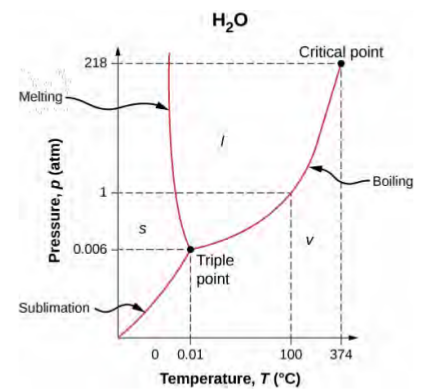
\includegraphics[width=0.5\textwidth]{figures/PT.png}
\caption{\label{fig:pt} \textit{Phase transitions} occur when crossing the lines.  Boiling, melting, and sublimation are the three possible processes.}
\end{figure}
\end{frame}

\begin{frame}{Temperature, Heat, and the 0th Law of Thermodynamics}
Snow \textit{sublimation}: \\ \vspace{0.5cm}
\url{https://youtu.be/8gh29dV-glI}
\end{frame}

\begin{frame}{Temperature, Heat, and the 0th Law of Thermodynamics}
A pressure cooker contains water and steam in equilibrium at a pressure greater than atmospheric pressure.  How does this greater pressure increase cooking speed?
\begin{itemize}
\item A: Raises the boiling point
\item B: Raises the vapor pressure
\item C: Both A and B
\item D: Changes the heat capacity of water and steam
\end{itemize}
\end{frame}

\begin{frame}{Temperature, Heat, and the 0th Law of Thermodynamics}
Triple point explained: \\ \url{https://www.youtube.com/watch?v=MP6MVLWuNZQ}
\end{frame}

\begin{frame}{Temperature, Heat, and the 0th Law of Thermodynamics}
\begin{figure}
\centering
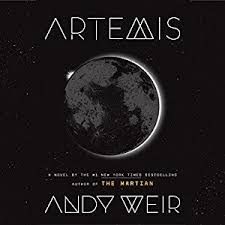
\includegraphics[width=0.5\textwidth]{figures/artemis.jpg}
\caption{\label{fig:artemis} Idea for bonus paper or group project: read \textit{Artemis} by Andy Weir and pick a chapter.  Explain each of the statements about surviving on the moon with lower artifical \textbf{vapor pressure}, artificial \textbf{boiling point}, no atmosphere, and a different $g$ value, etc.}
\end{figure}
\end{frame}

\begin{frame}{Temperature, Heat, and the 0th Law of Thermodynamics}
\small
During a phase transition, the temperature of a substance does not change.  The heat energy required to drive the phase transition is just proportional to the mass, for liquids and solids:
\begin{align}
Q &= m L_{\rm f} \\
Q &= m L_{\rm v}
\end{align}
These coefficients are known as the laten heats of \textit{fusion} and \textit{vaporization}.  These numbers have a molecular interpretation.
\end{frame}

\begin{frame}{Temperature, Heat, and the 0th Law of Thermodynamics}
\begin{figure}
\centering
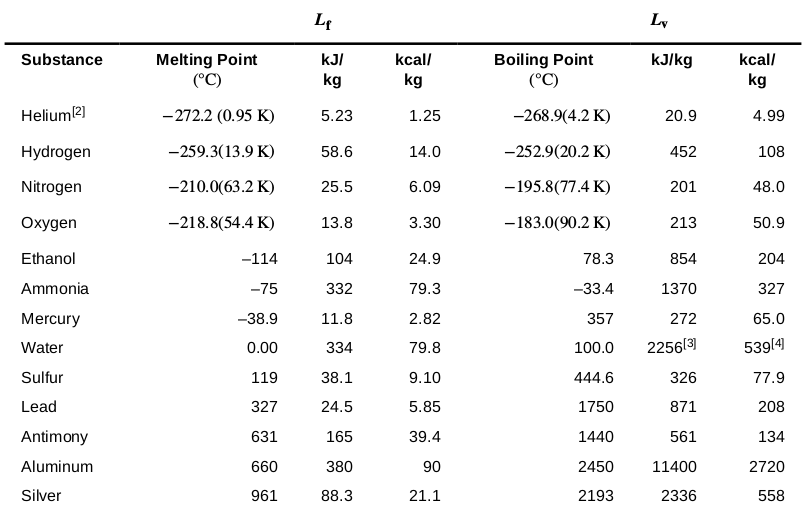
\includegraphics[width=0.9\textwidth]{figures/lvlf.png}
\caption{\label{fig:lvlf} As usual, look at water! (and aluminum).}
\end{figure}
\end{frame}

\begin{frame}{Temperature, Heat, and the 0th Law of Thermodynamics}
Three ice cubes are used to chill a soda at 20 $^\circ$C with mass 0.25 kg. The ice is at 0 $^\circ$C and each ice cube has a mass of 100.0 g. Assume that the soda is kept in a foam container so that heat loss can be ignored and that the soda has the same specific heat as water. Find the final temperature when all ice has melted.
\textbf{Group board exercise}: Latent heat of fusion of the ice: 334 kJ/kg, and heat capacity of water: 4186 J/kg/C.
\end{frame}

\section{Heat Capacity of Water, Latent Heat of Fusion of Water}

\begin{frame}{Heat Capacity of Water, Latent Heat of Fusion of Water}
\small
\textbf{Lab activity:} We are going to toss some ice into boiling water and measure the final temperature.  \textit{Choose the correct scale: calories, grams and degrees Celsius.} \alert{The specific heat of water is 1.0 calorie/gram/degree Celsius}.
\begin{enumerate}
\item Items: A thermometer, two small cups and one large cup, a scale, some ice, and some boiling water.
\item Measure the mass of each cup.
\item Pour some ice into one of the small cups and measure the mass of the ice.
\item Pour boiling water into the other small cup and measure the mass.
\item Mix them in the large cup, and wait until equilibrium is reached.
\item Measure the final temperature of the water/melted ice mixture.
\end{enumerate}
\end{frame}

\begin{frame}{Heat Capacity of Water, Latent Heat of Fusion of Water}
\small
\textbf{Lab activity:} We are going to toss some ice into boiling water and measure the final temperature.  \textit{Choose the correct scale: calories, grams and degrees Celsius.} \alert{The specific heat of water is 1.0 calorie/gram/degree Celsius}.
\begin{enumerate}
\item Using the initial and final temperatures of the ice and water, and the specific heat of water, measure the \textit{latent heat of fusion} $L_{\rm F}$ of ice.
\item $L_{f,ice} = c_{\rm w} \left( \frac{m_{\rm water}}{m_{\rm ice}} (T_{\rm i,H20} - T_{\rm f}) - T_{\rm f} \right)$
\item Expected value: 334 kJ/kg = 334 J/g
\item Collect handout on error analysis.  Use the handout to compute the average class value of latent heat of water, with proper statistical errors.  \textit{Review next class period.}
\end{enumerate}
\end{frame}

\section{JITT - Reading Quiz Results}

\begin{frame}{JITT 1.2}
\begin{enumerate}
\item What principle is used to determine the relationship between the internal energy of an ideal gas, and the temperature of the gas?
\item What principle or principles are used to determine the heat capacity of an ideal gas at constant volume?
\item The Maxwell-Boltzman distribution of molecular speeds gives the probability that a molecule will have a given speed in an ideal gas.  If it's not impossible for a molecule to have a speed of 0 m/s, why does this distribution go towards zero for v=0?
\end{enumerate}
\end{frame}

\begin{frame}{JITT 1.2}
\textbf{What principle is used to determine the relationship between the internal energy of an ideal gas, and the temperature of the gas?}
The ideal gas law. It relates the pressure and volume of the of a gas to its gas molecules (or number of moles of the gas) and the temperature of the gas.
\end{frame}

\begin{frame}{JITT 1.2}
\textbf{What principle is used to determine the relationship between the internal energy of an ideal gas, and the temperature of the gas?}
The temperature of molecules is used to determine the average kinetic energy of each molecule in a system. Then that kinetic energy is used to find the internal energy of an entire thermodynamic system. They use the equations $KE = \frac{3}{2}k_B T$ and $E_{int}=\frac{3}{2}Nk_BT$.
\end{frame}

\begin{frame}{JITT 1.2}
\textbf{What principle or principles are used to determine the heat capacity of an ideal gas at constant volume?}
Equiparition theorem.
\end{frame}

\begin{frame}{JITT 1.2}
\textbf{What principle or principles are used to determine the heat capacity of an ideal gas at constant volume?}
To determine the heat capacity of an ideal gas at a constant volume we use the principles of work and since there is no displacement, there is no work done and volume is constant. Using the formula for heat transfer, we set it equal to the amount of internal energy in the ideal gas, the resulting solution is $\frac{3}{2}R$.
\end{frame}

\begin{frame}{JITT 1.2}
\textbf{The Maxwell-Boltzman distribution of molecular speeds gives the probability that a molecule will have a given speed in an ideal gas.  If it's not impossible for a molecule to have a speed of 0 m/s, why does this distribution go towards zero for v=0?} \\
I don’t know.
\end{frame}

\begin{frame}{JITT 1.2}
\textbf{The Maxwell-Boltzman distribution of molecular speeds gives the probability that a molecule will have a given speed in an ideal gas.  If it's not impossible for a molecule to have a speed of 0 m/s, why does this distribution go towards zero for v=0?}
The distribution goes towards zero because the probability that a molecule will have exactly a given speed is 0.
\end{frame}

\begin{frame}{JITT 1.2}
\textbf{The Maxwell-Boltzman distribution of molecular speeds gives the probability that a molecule will have a given speed in an ideal gas.  If it's not impossible for a molecule to have a speed of 0 m/s, why does this distribution go towards zero for v=0?}
Because the probability of the molecules in a gas going 0 m/s is very low, thus the distribution heads to 0....A molecule slows down quicker and approaches zero quickly but never gets to it.
\end{frame}

\section{Mechanisms of Heat Transfer}

\begin{frame}{Temperature, Heat, and the 0th Law of Thermodynamics}
\textbf{Heat transfer mechanisms}:
\begin{itemize}
\item Conduction
\item Convection
\item Radiation
\end{itemize}
\end{frame}

\begin{frame}{Temperature, Heat, and the 0th Law of Thermodynamics}
\textbf{Conduction} - \textit{Heat transfer through stationary matter by physical contact.} \\ \vspace{0.5cm}
Which of the following do you think \textit{is not} an example of heat conduction?
\begin{itemize}
\item A: Accidentally touching a hot stove and feeling the burn
\item B: The sun shining on your face, making your face feel warm
\item C: Laying on hot sand on the beach, making you feel warm
\item D: A wire getting hot because it is carrying too much current
\end{itemize}
\end{frame}

\begin{frame}{Temperature, Heat, and the 0th Law of Thermodynamics}
\begin{figure}
\centering
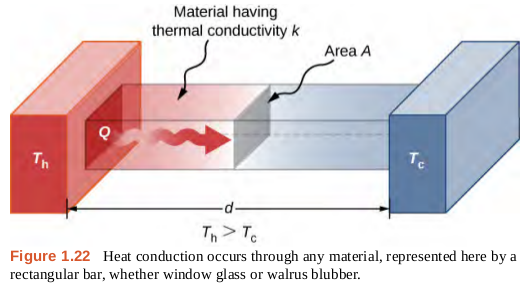
\includegraphics[width=0.7\textwidth]{figures/heat1.png}
\caption{\label{fig:heat1} Our model for heat transfer follows a differential equation.}
\end{figure}
\begin{equation}
P = \frac{dQ}{dt} = \frac{kA(T_{\rm h} - T_{\rm c})}{d} \rightarrow -kA \frac{dT}{dx}
\end{equation}
\end{frame}

\begin{frame}{Temperature, Heat, and the 0th Law of Thermodynamics}
\alert{Rate of conductive heat transfer}:
\begin{equation}
\boxed{
P = \frac{dQ}{dt} = \frac{kA(T_{\rm h} - T_{\rm c})}{d} \rightarrow -kA \frac{dT}{dx}}
\end{equation}
\begin{itemize}
\item \textit{k}: Thermal conductivity, W/m $^{\circ}$C
\item \textit{A}: Surface area in contact, m$^2$
\item \textit{d}: Thickness of contact area, m
\item \textit{$T_{\rm h}$, $T_{\rm c}$}: Hot and cold initial temperatures
\end{itemize}
The x-coordinate is the direction of heat flow and the minus sign reflects the corresponding decrease in temperature.  \textit{In American construction, sometimes $R = d/k$, known as the R-factor.}
\end{frame}

\begin{frame}{Temperature, Heat, and the 0th Law of Thermodynamics}
An aluminum can with thermal conductivity $k$ has a total area of $A$, and walls that are $x$ thick.  The soda in the can is much colder than the air outside, and a density $\rho$.  How much time passes before the soda is at the same temperature as the air?
\begin{itemize}
\item A: $t = \frac{\rho Vcx}{kA}$
\item B: $t = \frac{cx}{kA}$
\item C: $t = \frac{kAT}{x}$
\item D: $t = \frac{kAT}{x}$
\end{itemize}
\end{frame}

\begin{frame}{Temperature, Heat, and the 0th Law of Thermodynamics}
Why does the temperature difference not matter in the prior answer?
\begin{itemize}
\item A: Heat is not a rate, it's a substance
\item B: The aluminum does the heat conduction, not the soda
\item C: Energy conservation: the heat transferred does not depend on the initial and final temperature
\item D: The capacity of the air to absorb heat is much larger than the small can, so it happens as fast as possible
\end{itemize}
\end{frame}

\begin{frame}{Temperature, Heat, and the 0th Law of Thermodynamics}
Heat convection: we will not cover this quantitatively because it involves fluid dynamics. However, a good example is fur insulation against wind:
\begin{figure}
\centering
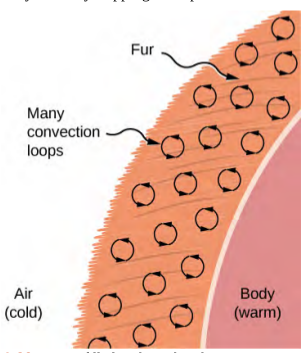
\includegraphics[width=0.4\textwidth,trim=0cm 0.1cm 0cm 0.1cm,clip=true]{figures/heat2.png}
\caption{\label{fig:heat2} Fur helps to insulate against wind chill.}
\end{figure}
\end{frame}

\begin{frame}{Temperature, Heat, and the 0th Law of Thermodynamics}
\small
Heat radiation: We can make one quantitative statement about radiative heat transfer.
\begin{figure}
\centering
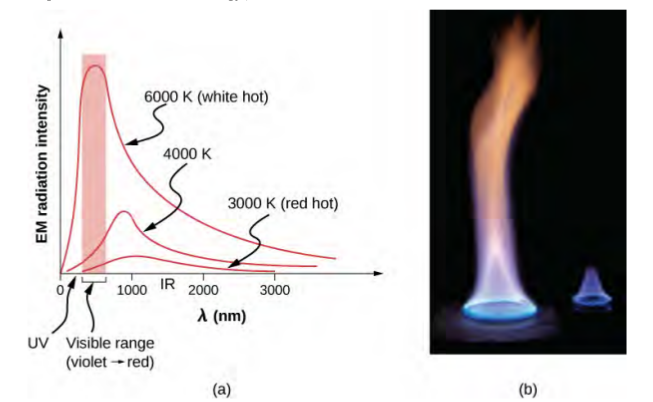
\includegraphics[width=0.6\textwidth]{figures/heat3.png}
\caption{\label{fig:heat3} Black-body radiation, where color depends on temperature.}
\end{figure}
\begin{equation}
P_{\rm net} = \sigma A e (T_{\rm 2}^4 - T_{\rm 1}^4)
\end{equation}
\end{frame}

\begin{frame}{Temperature, Heat, and the 0th Law of Thermodynamics}
\alert{The Stephan-Boltzmann} law of radiation
\begin{equation}
P_{\rm net} = \sigma A e (T_{\rm 2}^4 - T_{\rm 1}^4)
\end{equation}
\begin{itemize}
\item $\sigma$: Stefan-Boltsmann constant, $5.67 \times 10^{-8}$ W/(m$^2$ K$^4$)
\item $A$ is the surface area
\item $T_{\rm 1}$, $T_{\rm 2}$: temperatures of the object and environment
\item $e$: \textit{emissivity} of the object (can depend on the wavelength)
\end{itemize}
\end{frame}

\begin{frame}{Temperature, Heat, and the 0th Law of Thermodynamics}
This may sound like an odd question, but why do people need clothing?  Even if we are standing around in a room at room temperature, why do we get cold and get sick?
\begin{itemize}
\item A: The air conducts heat away from us if it is slightly colder
\item B: If there is a breeze, convection takes heat away from us
\item C: We naturally radiate heat in the infrared
\item D: All of these
\end{itemize}
\end{frame}

\begin{frame}{Temperature, Heat, and the 0th Law of Thermodynamics}
\textbf{Group board exercise}: Let's estimate the heat radiated by a person.  Use Stefan-Boltzmann law of radiation, with emissitivity of $1$ for infrared light.  Compare this to what you think is the natural amount of heat generated by a normal person's body (could start with 2000 Calories per day, for example).
\end{frame}

\begin{frame}{Temperature, Heat, and the 0th Law of Thermodynamics}
\small
Greenhouse effect as heat transfer problem: \\ \url{https://phet.colorado.edu/en/simulation/greenhouse}
\begin{itemize}
\item What is the CO$_2$ concentration in the previous ice age, and what temperature does this allow on the Earth's surface?  With clouds?
\item Repeat, but with the numbers of today.  Add clouds, and repeat.  Write down all the temperatures you think are the equilibrium temperatures.
\item Open the photon absorption tab.  Create three different atmospheres: all methane, all carbon dioxide, and all nitrogen.  What happens to the infrared photons in each?
\end{itemize}
\end{frame}

\begin{frame}{Kinetic theory of gases}
When we say the word "molecule," we take it for granted.  How do you actually know substances are made of molecules?  Can we know this by observing gases? \\ \vspace{1cm}
Chapter 2 leads us into the subject of the \alert{kinetic theory of gases}, acting on the hypothesis of the existence of molecules and drawing conclusions about the behavior of gases.
\end{frame}

\begin{frame}{Kinetic theory of gases}
After observations in the 16th-19th centuries (Boyle's Law, Charles's Law, Guy-Lussac Law), we arrived here: \\ \vspace{1cm}
\begin{equation}
\frac{p_1 V_1}{T_1} = \frac{p_2 V_2}{T_2}
\end{equation}
\begin{itemize}
\item p: pressure
\item V: volume
\item T: temperature
\end{itemize}
Suppose we guess that gases are made of smaller pieces, and that temperature is the experience of the flow of heat, and that heat is proportional to the kinetic energy of the smaller pieces.
\end{frame}

\begin{frame}{Kinetic theory of gases}
Let us name that last idea \textit{equipartition of energy}, that each \alert{degree of freedom} gets one piece of kinetic energy proportional to temperature:
\begin{equation}
e_{\rm dof} = \frac{1}{2}kT
\end{equation}
\begin{itemize}
\item T is the temperature of the gas of molecules
\item k, for now, is some constant
\item e is the energy per degree of freedom
\end{itemize}
\end{frame}

\begin{frame}{Kinetic theory of gases}
Suppose a molecule bounces off of a flat container.  What if pressure is just the collective force per unit area of molecules all bouncing around at the same time?  How do we describe this process with concepts from last semester?
\begin{itemize}
\item Elastic collisions, momentum conservation
\item Force in terms of momentum
\end{itemize}
\end{frame}

\begin{frame}{Temperature, Heat, and the 0th Law of Thermodynamics}
\small
\begin{figure}
\centering
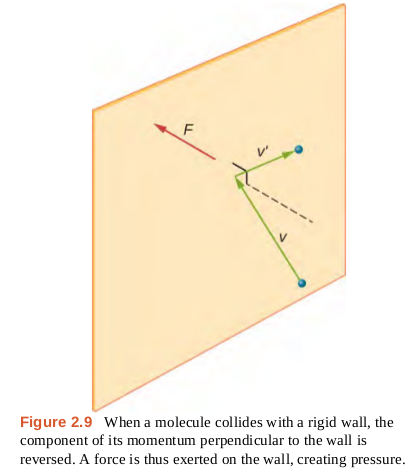
\includegraphics[width=0.4\textwidth]{figures/p1.png}
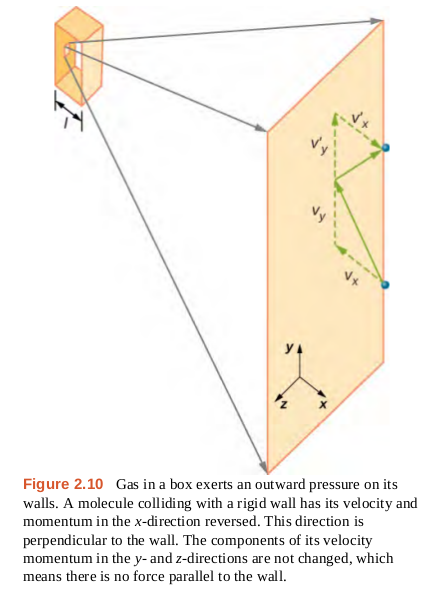
\includegraphics[width=0.4\textwidth]{figures/p2.png}
\caption{\label{fig:p1} The force imparted on the wall by a molecule with velocity $v$, then $v'$, causes pressure.  The box is a length $l$ and the molecule is assumed to travel all the way across.}
\end{figure}
\end{frame}

\begin{frame}{Temperature, Heat, and the 0th Law of Thermodynamics}
Assumptions:
\begin{itemize}
\item Large number $N$ of molecules with mass $m$.
\item Molecules are classical (Newton's laws)
\item Molecules are much smaller than the container and distance between each other
\item All collisions are elastic
\end{itemize}
\end{frame}

\begin{frame}{Temperature, Heat, and the 0th Law of Thermodynamics}
Momentum transfer of one molecule colliding with the wall: \\
\begin{equation}
F_i = (mv_{x} - m(-v_{x}'))/\Delta t = \frac{2mv_x}{\Delta t}
\end{equation}
The box has a length $l$:
\begin{equation}
F_i = \frac{2mv_x}{2l/v_x} = \frac{mv_x^2}{l}
\end{equation}
\end{frame}

\begin{frame}{Temperature, Heat, and the 0th Law of Thermodynamics}
Now let's account for all molecules:
\begin{equation}
F = \frac{m}{l}\Sigma_i^N v_x^2 = \frac{Nm}{l} \bar{v_x^2}
\end{equation}
(That's the \textit{average} of the squared velocity).  The x-direction is not special, so we may assume $\bar{v_x^2} = \frac{1}{3}\bar{v^2}$
\begin{equation}
F = \frac{Nm\bar{v^2}}{3l}
\end{equation}
And pressure is just force per surface area:
\begin{equation}
pA = \frac{Nm\bar{v^2}}{3l}
\end{equation}
Now we realize that $Al = V$...
\end{frame}

\begin{frame}{Temperature, Heat, and the 0th Law of Thermodynamics}
Now we realize that $Al = V$...
\begin{equation}
pV = \frac{Nm\bar{v^2}}{3} = \frac{2}{3} N \left(\frac{1}{2}\right) m \bar{v^2}
\label{eq:soHot}
\end{equation}
Now, use the \textit{equipartition theorem}, assuming three degrees of freedom per molecule (three dimensions of velocity):
\begin{equation}
\bar{K} = \frac{3}{2}kT
\end{equation}
Substituting the kinetic energy into Eq. \ref{eq:soHot}, we find
\begin{equation}
\boxed{
pV = NkT}
\end{equation}
The Ideal Gas Law.
\end{frame}

\begin{frame}{Temperature, Heat, and the 0th Law of Thermodynamics}
We need a new unit, a new \textit{scale}, since the number of molecules is so large.  How about the number of carbon atoms in 12 grams of carbon-12 (the most common isotope)? \\ \vspace{0.5cm}
Let's call the number of molecules $N_{\rm A}$ in 12 grams of carbon a \alert{\textit{mole}}, and let $n = N/N_{\rm A}$.  If the \alert{Gas constant} $R = kN_{\rm A}$, then the Ideal Gas Law says
\begin{equation}
pV = nRT
\end{equation}
where $n$ is the number of moles and $R = kN_A = 8.31$ J/mole/Kelvin $\approx 2$ cal/mole/Kelvin.
\end{frame}

\begin{frame}{Temperature, Heat, and the 0th Law of Thermodynamics}
Guess what's about to happen?  A ton of problems with the Idea Gas Law?  You're right! \\ \vspace{0.5cm}
If we have a \textit{1 liter} ($10^{-3}$ m$^3$) vessel of argon at a temperature of 300 K, what should the pressure be, if there are only 0.3 moles in the vessel?
\begin{itemize}
\item A: 0.2 atm
\item B: 2 atm
\item C: 20 atm
\item D: 200 atm
\end{itemize}
\end{frame}

\begin{frame}{Temperature, Heat, and the 0th Law of Thermodynamics}
How many air molecules are in a liter of air? ($p = 1$ atm = 100 kPa, $V = 10^{-3}$ m$^3$, $R = 8.31$ J/mole/Kelvin, $T = 300$ K).
\begin{itemize}
\item A: $3 \times 10^{21}$
\item B: $3 \times 10^{22}$
\item C: $6 \times 10^{21}$
\item D: $6 \times 10^{22}$
\end{itemize}
Precise measurement of Avogadro's Number $N_A = 6.02 \times 10^{23}$ molecules.
\end{frame}

\begin{frame}{Temperature, Heat, and the 0th Law of Thermodynamics}
PhET Simulation:
\url{https://phet.colorado.edu/en/simulation/gas-properties} \\ \vspace{0.5cm}
I would like you to measure \textbf{\alert{Boltzmann's Constant, $k_{\rm B}$}}, using the idea gas law and the PhET simulation.
\begin{itemize}
\item $pV = Nk_{\rm B}T$
\item $N$ is calibrated on right side
\item $p$ and $T$ are measurements
\item Assume $V = Al$.  The ruler can measure $l$, and assume $A$ is (35 nm)$^2$.
\item You can independently adjust the temperature by adding heat at the bottom.
\end{itemize}
Separately, confirm Boyle's Law and Charles's Law.
\end{frame}

\begin{frame}{Temperature, Heat, and the 0th Law of Thermodynamics}
\textbf{\alert{Boltzmann's Constant, $k_{\rm B}$}} is related to the gas constant $R$ by $R = N_{\rm A} k_{\rm B}$.  Electrochemical measurements and Brownian motion measurements (\textit{paper idea}) tell us that $N_{\rm A} = 6.02 \times 10^{23}$.  So $R$ involves cancellation of many orders of magnitude to have the value of 8.31 in SI units...
\end{frame}

\begin{frame}{Temperature, Heat, and the 0th Law of Thermodynamics}
Modification to Idea Gas Law: known as van der Waals equation of state.
\begin{equation}
\left(p + a \left(\frac{n}{V}\right)^2\right)(V-nb) = nRT
\end{equation}
\begin{itemize}
\item a and b are empirical constants
\item Same temperature for a lower pressure $\rightarrow$ molecular attractions
\item Corrects for high density gases in which the molecule volume matters
\end{itemize}
\end{frame}

\begin{frame}{Temperature, Heat, and the 0th Law of Thermodynamics}
\small
\begin{figure}
\centering
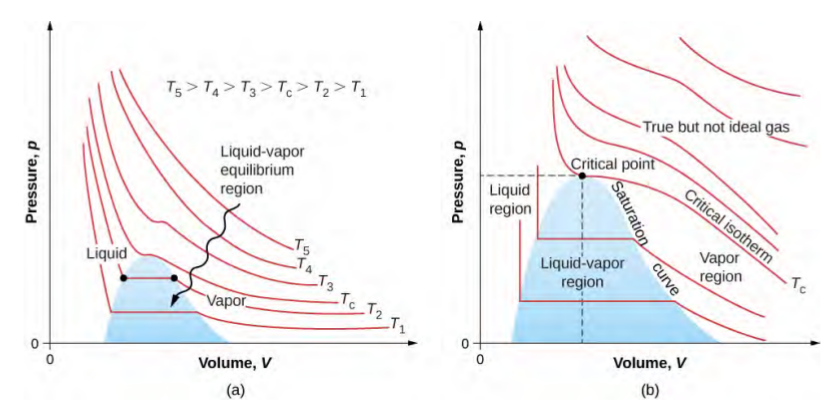
\includegraphics[width=0.9\textwidth]{figures/p3.png}
\caption{\label{fig:p3} The van der Waals equation of state leads to more realistic isotherms, and probes the liquid-vaper region near the critical point.}
\end{figure}
\end{frame}

\begin{frame}{Temperature, Heat, and the 0th Law of Thermodynamics}
\textbf{Heat capacities of gases}: As we saw from the PhET simulation activity, we cannot just change the temperature of a gas without either the pressure or the volume changing.  To understand heat flow into gases, we need to hold these constant (theoretically).  Recall that the average energy for a molecule in a gas is 
\begin{equation}
E_{\rm int} = \frac{3}{2}nRT
\end{equation}
Let the \textit{molar heat capacity at constant volume} be defined in a similar way to solids:
\begin{equation}
C_{\rm V} = \frac{1}{n}\frac{Q}{\Delta T}
\end{equation}
\end{frame}

\begin{frame}{Temperature, Heat, and the 0th Law of Thermodynamics}
Combining these two equations, we find  
\begin{equation}
C_{\rm V} = \frac{3}{2}R
\end{equation}
$C_{\rm V}$ is independent of temperature, merely a constant of nature for idea gases. However, note that we only find the number $\frac{3}{2}$ because of the equipartition theorem while assuming only three degrees of freedom.  If we had identified more degrees of freedom, we would have drawn a different conclusion.
\end{frame}

\begin{frame}{Temperature, Heat, and the 0th Law of Thermodynamics}
\small
\begin{figure}
\centering
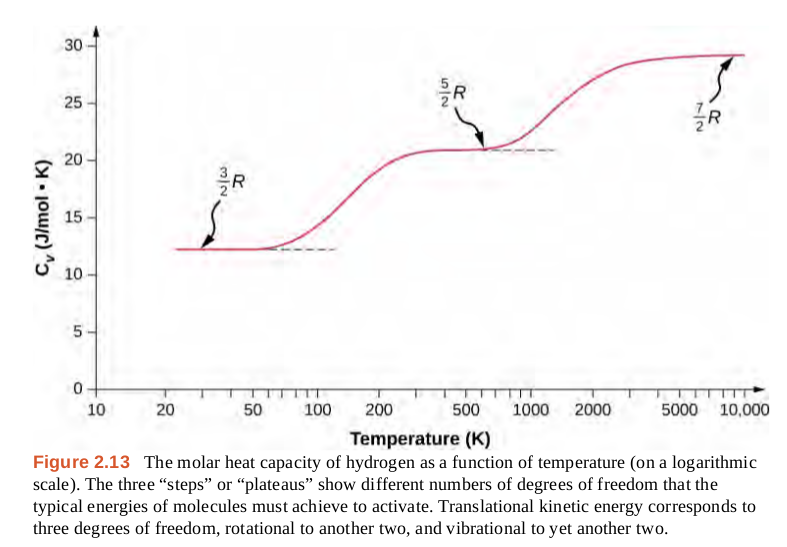
\includegraphics[width=0.8\textwidth]{figures/cv.png}
\caption{\label{fig:cv} $C_{\rm V}$ for H-gas reveals molecular (atomic) nature of the gas.  The right-most temperatures correspond to a few percent of 1 Rydberg energy.}
\end{figure}
\end{frame}

\section{Conclusion}

\begin{frame}{Unit 1 Summary}
\textbf{Reading: Chapters 1 and 2}
\begin{enumerate}
\item Temperature, Heat, and the 0th Law of Thermodynamics
\item Heat flow and transfer mechanisms
\item Kinetic Theory of Gases
\end{enumerate}
\end{frame}

\section{Answers}

\begin{frame}{Answers}
\small
\begin{columns}[T]
\begin{column}{0.5\textwidth}
\begin{itemize}
\item Momentum and kinetic energy are conserved for each molecule
\item $2mv$
\item $\alpha\exp(\alpha t)$
\item $\exp((\alpha+\beta) t)$
\item The increase is smaller than 10 degrees in $^{\circ}$C
\item The increase is the same in $^{\circ}$K
\item $35^{\circ}-40^{\circ}$C is comparable to human body temperature
\item Answer B
\end{itemize}
\end{column}
\begin{column}{0.5\textwidth}
\begin{itemize}
\item 1 mm
\item -10 MPa
\item A and B
\item Cannot determine (would have needed the heat capacity of water)
\item The temperature change corresponding to system 2
\item The changes corresponding to system 1 and 2 are equal
\item Higher by a factor of 4
\item Both A and B
\end{itemize}
\end{column}
\end{columns}
\end{frame}

\begin{frame}{Answers}
\small
\begin{columns}[T]
\begin{column}{0.5\textwidth}
\begin{itemize}
\item The sun shining on your face, making your face feel warm
\item $t = \frac{\rho Vcx}{kA}$
\item Energy conservation: the heat transferred does not depend on the initial and final temperature
\item 20 atm
\item $3 \times 10^{22}$
\end{itemize}
\end{column}
\begin{column}{0.5\textwidth}
\end{column}
\end{columns}
\end{frame}

\end{document}
